%*******************************************
\section{Evaluation}
%*******************************************
\label{s:evaluation}
\textbf{VLL FORMS IN APPENDIX? }As a final step the Anti-Phishing Education we have designed and implemented needs to be evaluated which is the goal of this chapter.
 The app will be evaluated with the aid of a user study.
 After introducing our study design, we will state our hypothesis and explain how we are going to measure our statements in order to prove that they are true or false.
 Finally, we will analyze our results and state our conclusion.


%===========================================
\subsection{Participant Recruitment}
%===========================================
%Oder was soll hier rein? ;)
%osn - freundes freunde
%telefon -freundes freunde
%flyer ausgeteilt
%flyer per e-mail an sehr viele professoren geschickt und gebeten weiter an studenten zu leiten
%ein paar leute auf der straße angesprochen - da erfolglos
%Verlosung eines amazin gutscheins


%===========================================
\subsection{Study Design}
%===========================================
For time reasons and lack of participants we decided to run a "Before and After App" Study with the same groups of people.
 Specifically, our user study is structured as follows:

\begin{enumerate}
	\item \textbf{General Before-Survey} At the beginning the participants have to fill out a general survey, where they have to judge their own knowledge on the topic of Internet security in general.
 For instance, they are asked whether it is easy for them to distinguish legitimate e-mails and websites from fake ones.

	\item \textbf{Website-Survery Before} In this part of the user study the participants gets a list of screenshots of websites.
 The screenshots had been taken with the standard browser of an Android tablet.
 In total, the user is shown 16 screenshots, with 8 phishing and 8 valid URLs.
 The user has to decide whether he would enter confidential data on the shown website.
 Additionally, he has to encircle the part of the screenshot which was the primary reason for his decision.
 Then, the user has to indicate how sure he was about his answers on a Likert scale.
 Finally, the user is asked whether he knows the vendor of the website and whether he has a account there.

	\item \textbf{Play App} After the "Website-Survey Before" the users get the smartphones in order to play the app.
 To save time, we skipped the introduction 2 part ("access address bar") for the user study.
 The user has half an hour to play the app.
 After half an hour they are asked to put the smartphones aside.
 Then, we collect the smartphones and note the reached points in each level.

	\item \textbf{Website-Survery After} After playing the app, the participants get a second website-survey.
 In this, all examples of the previous survey are included.
 Moreover, it contains 8 further website screenshots of which 4 have phishing and the remaining 4 have valid URLs.

	\item \textbf{General After-Survey} Finally, the participants are asked to fill out a form with questions to their demographics.
 This form does also contain questions related to the SUS and some other questions regarding their impression of the app.



\end{enumerate}

%===========================================
\subsection{Hypotheses}
%===========================================
In order to evaluate the effectiveness and usability of our app we have formulated the following hypotheses for the user study:

\begin{enumerate}
	\item \textbf{Hypothesis 1 - Mistakes} After playing the app, the users make significantly less mistakes in detecting phishing websites compared to before playing the app.

	\item \textbf{Hypothesis 2 - URL Based Decision} After playing the app, the users base their primary decision on whether a website is a phishing website or not significantly more often based on the URL compared to before playing the app.

	\item \textbf{Hypothesis 3 - URL Comprehension} After playing the app the user understands the importance of the second- and top-level domain of a URL as the only criteria to detect phishing websites.

	\item \textbf{Hypothesis 4 - Good Usability} The app is easy to understand and to use.

\end{enumerate}


%===========================================
\subsection{Measurement}
%===========================================
In the following we will elaborate on how we are going to measure the statements of our hypothesis and show that they are true or false.


\begin{enumerate}
	\item \textbf{Hypothesis 1 - Mistakes} Correct answers in "Website-Survery After" $>>$ correct answers in "Website-Survery Before" 
	\item \textbf{Hypothesis 2 - URL Based Decision} Number of URL markings in "Website-Survery After" $>>$ number of URL markings in "Website-Survery Before" 
	\item \textbf{Hypothesis 3 - URL Comprehension} Number of marked second- and/or top-level domains of URLs in "Website-Survery After"  $>>$ number of marked second- and/or top-level domains of URLs in "Website-Survery Before" 
	\item \textbf{Hypothesis 4 - Good Usability} System Usability Scale (SUS) $>$ 68
\end{enumerate}

%===========================================
\subsection{Results and Analysis}
%===========================================
\subsubsection{interpretation problems}
\label{s:intprobs}

\subsubsection{Analysis of our hypotheses}
\label{s:hypanalysis}

\begin{figure}
\centering
\subfigure[Before]{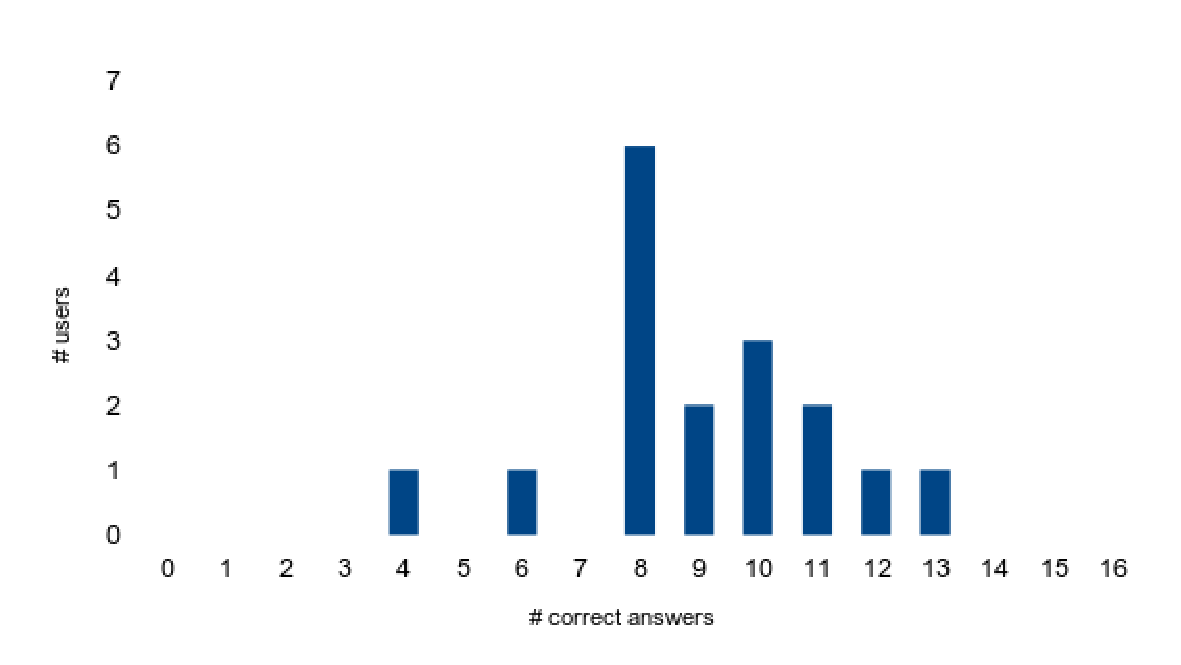
\includegraphics[width=0.45\textwidth]{hyp1b.pdf}}
\subfigure[After (all URLs)]{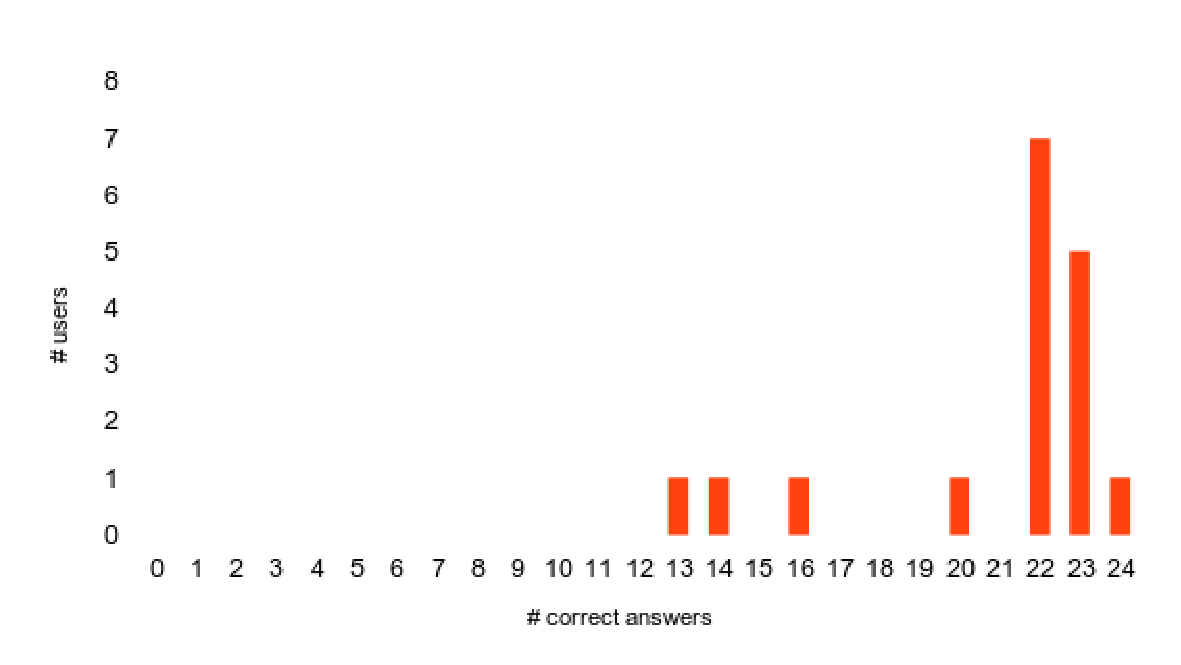
\includegraphics[width=0.45\textwidth]{hyp1a.pdf}}
\subfigure[After (New URLs)]{\label{fig:hyp1resultsanew}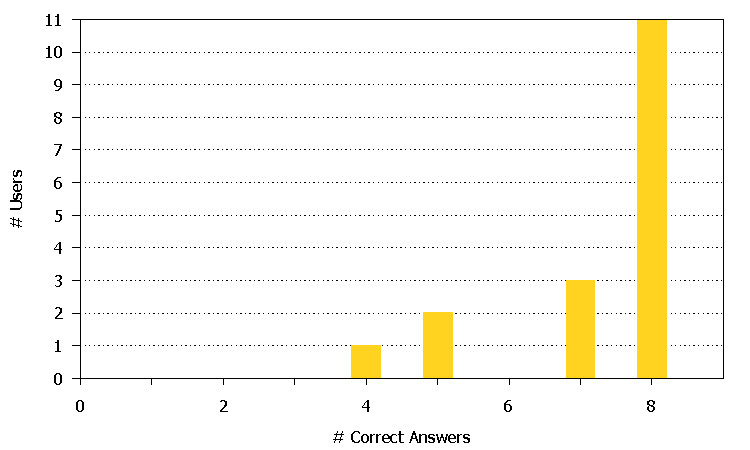
\includegraphics[width=0.45\textwidth]{hyp1anew.pdf}}
\subfigure[After (Repeated URLs)]{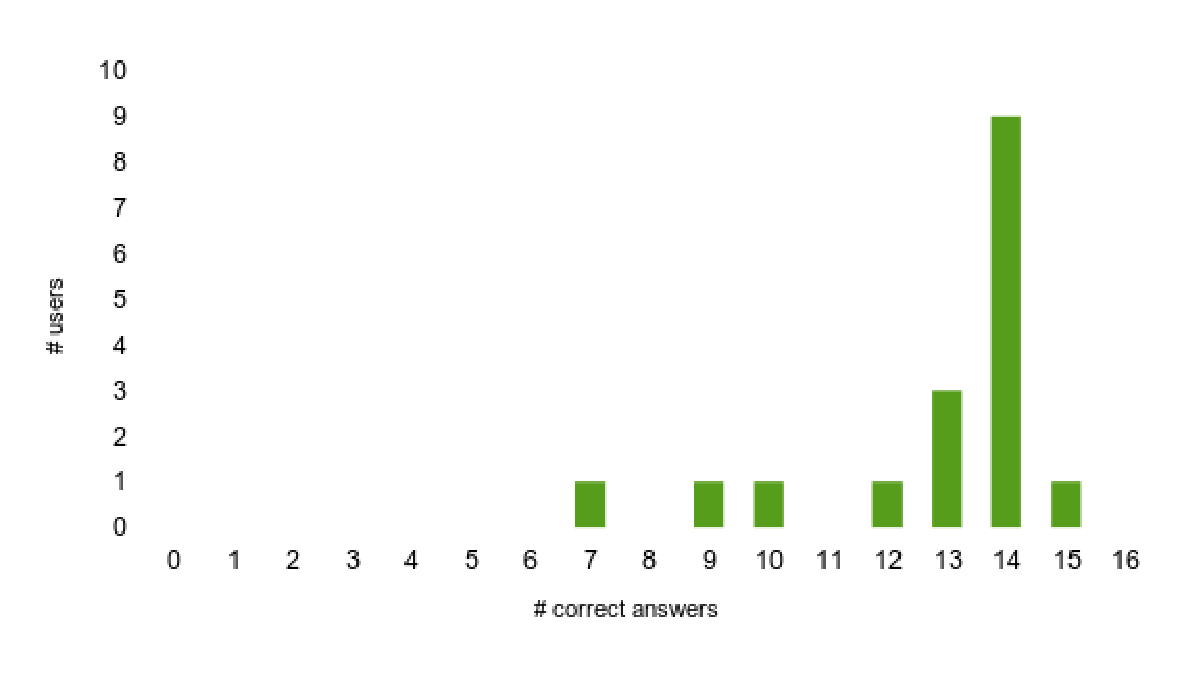
\includegraphics[width=0.45\textwidth]{hyp1arepeat.pdf}}
\caption{Correct Answers}
\label{fig:hyp1results}
\end{figure}

\begin{figure}
\centering
\subfigure[Before]{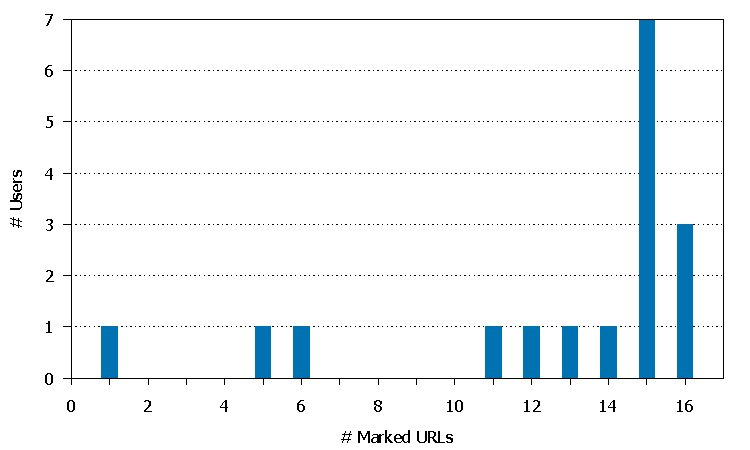
\includegraphics[width=0.45\textwidth]{hyp2b.pdf}}
\subfigure[After]{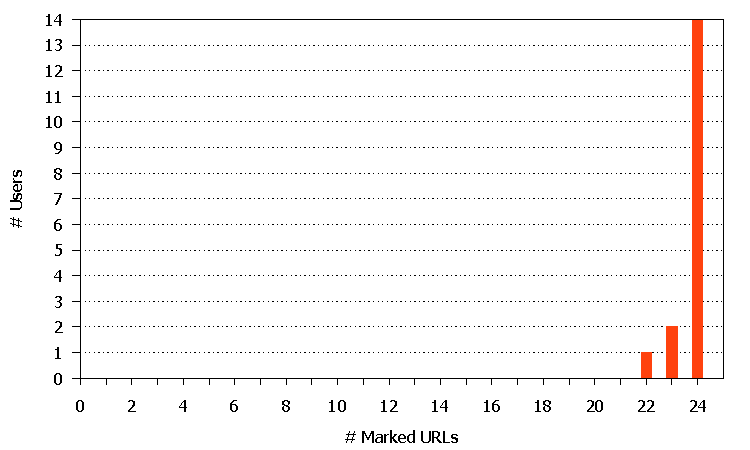
\includegraphics[width=0.45\textwidth]{hyp2a.pdf}}
\caption{URL marked}
\label{fig:hyp2results}
\end{figure}

\begin{figure}
\centering
\subfigure[Before]{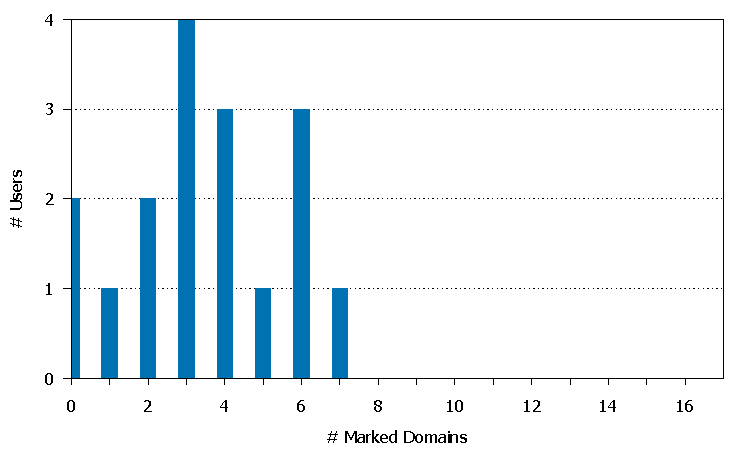
\includegraphics[width=0.45\textwidth]{hyp3b.pdf}}
\subfigure[After]{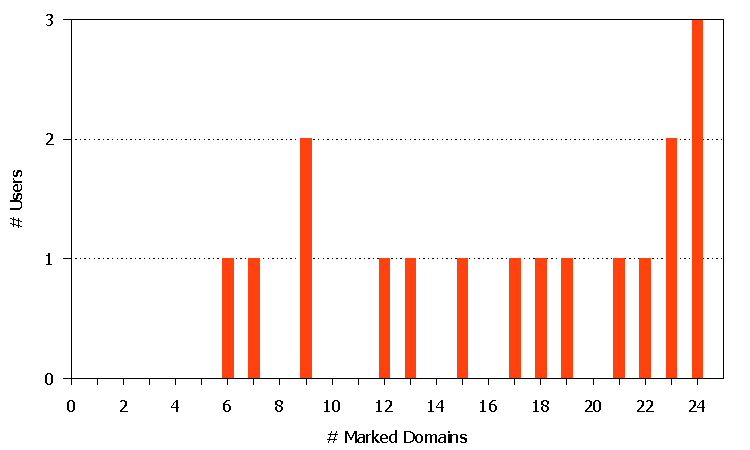
\includegraphics[width=0.45\textwidth]{hyp3a.pdf}}
\caption{Domain marked}
\label{fig:hyp3results}
\end{figure}

\begin{description}
\item[Hypothesis 1]
\autoref{fig:hyp1results} shows the results of our study according to hypothesis 1. One can clearly see that the majority of the users identified more URLS correctly after using the app than before. While most participants correctly identified 8 out of 16, i.e. 50\%, websites before they played the app, the majority gave correct answers to 22 out of 24 websites afterwards, i.e. 91.67\%. One could argue that this increase is based on the fact that the examples are mainly the same. \autoref{fig:hyp1resultsanew} however shows that the user also got most of the new URLs right. Therefore we assume that we can furthermore ignore this learning effect. 
\item[Hypothesis 2]
\autoref{fig:hyp2results} shows how many users marked the URL as their main source of decision.
Most of the users already based most of their decisions on the URL before.
Occasionally users marked the content or the padlock.
However only 3 Users (17.65\%) always marked the URL.
Afterwards we see that most users (82.35\%) always based the decision on the URL and only 3 Users made on or two mistakes.
Therefore we think that our app emphasized their believe in basing their decision on the URL.
We however think it is important to tell the user this to get uncertain or unknowing users to the same level as most of our participants.
Also our app empathizes the importance of the URL by putting the main focus on it.
We have decided against doing statistical test on this hypothesis.
We believe it will most likely be rejected because the change from before to after is not very high.
\item[Hypothesis 3]
There is a general problem with the question in the websites-before-survey.
We were not able to clearly ask the user to mark the Domain when it was the base of their decision because we would have then primed them to look at the URL or even the Domain.
This would have influenced the results of Hypothesis 2.
Therefore a user might mark the whole URL even if his decision was based only a small part (e.g. the Domain) of the URL.
We where aware of this problem beforehand but saw no other option than to formulate the question in such an open form.
Because of this we can not clearly identify what their main source of decision was in the before survey.
Afterwards the user knew that we wanted them to mark the domain.
This can be interpreted as a change of question even if the literal question did not change.
Therefore we can not apply any statistical tests on this Hypothesis.
Nevertheless none of the users marked the domain in most cases beforehand, i.e. 7 domains out of 16 URLs where marked at most by only one user.
\begin{figure}
\centering
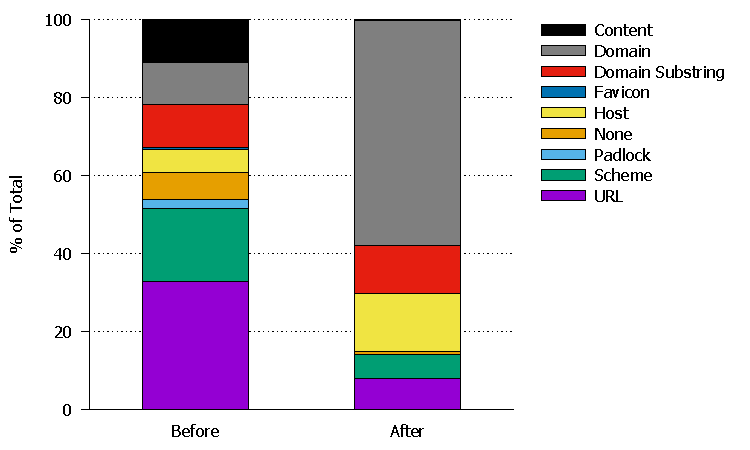
\includegraphics[width=0.45\textwidth]{markings.pdf}
\caption{Marked parts of the screenshot before and after.}
\label{fig:markings}
\end{figure}
\autoref{fig:markings} shows the distribution of the marked areas before and after. One can clearly see that afterwards most of the users marked the domain. However we are not able to compare that to the before values because of the changed question.
\item[Hypothesis 4]
\end{description}


\subsubsection{Further Exploration}
Some of the results can not be proven statistically, mainly because of the low sample count. 
Therefore, we only exploratively analyze these results in this section.
textbf{In this section we consider all of our participants. do we????} 

\begin{description}[leftmargin=0cm]
	\item[text]
\end{description}


During playing the app, the participants had a slip of paper for notes they wanted to make considering the app.
In the following we outline the main results of these slips of paper.
Note that we did not ask the users to write down something specific. 
We merely asked them to write down what they thought, i.e. there might be more participants who agreed with some of these points below but just have not explicitly written it down.
\textbf{Wenn nicht oben, dann hier auf jeden fall alle betrachten}.

\begin{description}[leftmargin=0cm]	
	\item[Scrolling of URL] In addition to deciding whether a URL is a phish or not, the user has to face two more 	challenges. 
First, the font size gets increasingly smaller in higher levels, until it eventually is approximately the same size of the Android standard browser.
Second, the URL is displayed in a horizontal scrollbar so that he has to scroll the URL to the right in order to view the beginning of it, just like it is the case in browsers.
4 of our 19 participants (21\%) found this disturbing and said it hindered them from analyzing the URL reasonably. 
Well, this is exactly what we wanted, since the behavior in the browser is the same, and users should practice it.
We assume that the users would not have noted this in this extent in case they would have had to complete introduction 2 (access the address bar), because then they would have understood why we do the URL scrolling.
Yet, we think after a couple of levels the users should have understood that they have to scroll the URL, in the game as well as in the browser, so one might consider to eliminate after some time. 
	\item[Unknown Services] We have mentioned the problem of unknown services in \autoref{s:problems_with_URLs}.
As we were afraid there are in fact services which are not familiar to several users.
4 out of 19 participants (21\%) mentioned this problem.
Even if we tried to make use of the most popular services with the aid of Alexa's~\cite{alexa} ranking we cannot assure that all used URLs are known by all users.
One idea to approach this challenge might be to provide an question mark button in addition to the check mark (no phish) and cross mark (phish) buttons. 
When a player clicks on this button, he can be told whether the given URL is a phish or not and why.
From this action the user would neither profit nor would he lose any points or lives.
Yet, we do not think that this is a major issue, since the users got at least until level 4 and most of them achieved even higher levels.
We are confident that the app in its current state is already implicitly able to teach the users about the legitimacy of unknown services.
After facing unfamiliar URLs and making or not making mistakes they will eventually learn whether to trust a service or not.
	\item[Question to Data Entry] Originally, the website-surveys before and after asked the participants whether they thought a given website screenshot was a phishing website or not.
After our test iteration of our study, however, we decided to change the question towards asking the user whether they would enter their personal data into this website in order to create some context for the user. 
As we told the user that this study was particularly about phishing and that their task was to detect phishing websites in the website-surveys before and after, we believe that it was clear what we were asking for with this question.
Yet, 3 participants (15.8\%) noted that the formulation of this question was unclear, i.e. there might have been participants who selected ``no'' even if they did not think it was a phishing website, but they would  generally not enter their data in this website.
	\item[Explanations and Comprehensibility]
4 participants (21\%) stated on their slips of paper that they found the explanations of the app very good and easy to understand.
1 of these 4 participants, however, added that there is partially much text to read.
Another participant (not under those 4) noted that there is too much and long text in general.
	\item[App Structure]
We did our best to develop an app which is consistent and well-structured.
3 of our participants (15.8\%) confirmed our intentions by stating that they found our app well and clearly-structured.
	\item[Button Positioning] The positioning of our app buttons during the game are as follows: 
The left bottom corner has a check mark which represents that the user thinks the displayed URL is not a phish.
The right bottom corner has a cross mark which means that the user thinks the displayed URL is a phish.
After clicking on either of these buttons in the write bottom corner another button appears (where the cross mark usually is) which either is the continue or the verify button (depending on whether the user has to select the Who-Section or not).
2 of our participants (10.5\%) indicated that the positioning of the buttons in the right bottom corner are suboptimal.
The problem here is that accidentally double clicking, for example, the continue button in the right corner results in rejecting the next URL even if the user might not have intended to.
Even if only 2 participants explicitly criticized this aspect we believe that this is a legitimate point.
In fact, the positioning of the two buttons continue and verify should be different from the one of the cross mark.
This is an aspect which should be targeted in future work. 
	\item[Repetition]
Repetition is an important element of our app.
In every level introduction we briefly repeat the so far learnt parts of a URL (with a graphic) and the different attacks the user has seen until this point.
We also make use of repetitions during the exercise rounds, every level contains at least one exercise from the previous level.
2 of our participants (10.5\%) explicitly indicated that our repetitions made them feel more confident and safer.
	\item[External Links]
In the main menu of our app we have a button ``More About Phishing'' which leads to a list of external links to various websites about phishing.
As it is often easier to find websites on a specific topic in English, some of these websites are in English as well.
2 participants (10.5\%) indicated that they did not like it to be led to an English website and would have expected to be forwarded on a German one.
This aspect is also a point which is worth to consider for future work, since we cannot expect our audience to have knowledge of the English language.
An idea to approach this might be to provide in-app additional info.
That is, instead of linking to external websites, the app itself could provide additional categorized information in German.
This would solve the problem with the language and at the same time the additional information would fit to our app layout and design.
	\item[Amount of Examples] Our app starts with a small sample of URLs users have to decide on.
In every level the sample size increases as the number of possible attacks increase.
2 participants (10.5\%) found that our sample size was to big.
This might have been the result of the fact that the users had to play the game for half an hour at a time.
Yet, re-thinking the number of URLs per level might be reasonable, but one has to consider that there have to be enough phishing URLs for the repetition as well as the new attack in each level.
	\item[Mail Not Received] The first part of our app includes sending a spoofed e-mail to oneself in order to increase the awareness of how easy faking e-mails is, even for unexperienced users.
1 participant did not receive the e-mail he tried to send to himself.
He skipped this part by clicking on the according button we had added for such cases.
All other participants received the spoofed e-mail.
	\item[Further Suggestions] In their notes some users made several suggestions which we found interesting and would like to mention here.
2 participants stated that the attacks in level 2 are not very challenging and very obvious.
Phishing URLs are of the following kind in this level: ``http://www.ebay.de.phisher.com/login''.
We had done this intentionally, however maybe the app could in fact start with for example nonsense attacks or just reduce the number of samples in this level.

Another participant noted that the repeating sentences ``Very good. You are now a bit safer'', for example, when the user correctly identified a phish, were kind of repetitive and not motivating enough. This is ultimately related to our issue with the Law~of~Effect in \autoref{s:learning_principles}.
There we stated that the texts and icons of the app should vary according to the user's performance and the degree of difficulty in order to achieve higher and better positive feelings.
This is an additional point which is worth to consider for future work.

A participant would have wished more ``feedback'' on his progress in general. 
He missed statistics, highscores or other forms of long-term feedback.
As we mentioned in \autoref{s:learning_principles} and \autoref{s:game_techniques} feedback is essential for learning as well as games.
For this reason, this aspect is something which should be enhanced in future.

A further interesting point is that one of our participants noted that he thought our app was appropriate for schools.
From this we infer that the participant found our app easy to understand and that he thought pupils were capable of understanding and playing our app.
In fact, this is a very good and important point.
People might not want to learn about phishing on their own, especially pupils would probably not think about that.
However, if computer security is a part of the education plan and if pupils have to learn something about, for example, phishing by playing the app, a far larger audience can be reached and educated on this topic.	
\end{description}
%===========================================
\subsection{Discussion}
%===========================================
%===========================================
\subsection{Conclusion}
%===========================================
